
\documentclass{pnastwo}
\usepackage{graphicx}
\usepackage{amsmath}

\begin{document}
	
	
\title{The relationship between scaled selection coefficients and dN/dS}
	
\author{Stephanie J. Spielman\affil{1}{Department of Integrative Biology, Center for Computational Biology and Bioinformatics, and Institute of Cellular and Molecular Biology.
		The University of Texas at Austin, Austin, TX 78712, USA.} 
	\and
	Claus O. Wilke\affil{1}{}
}
	
\contributor{Submitted to Proceedings of the National Academy of Sciences of the United States of America}
\maketitle

\begin{article}
		
\begin{abstract} %PNAS - 250 words. We are currently at 242.
Inferring the strength of natural selection in protein-coding sequences along a phylogeny is a major objective in the field of molecular evolution. Two broad classes of Markov-process models have been developed to describe these selective pressures. The first and most widely-used variety, mechanistic codon (MC) models, estimate the evolutionary rate ratio $dN/dS$ and have been developed to a high level of sophistication. The second class of models, known as mutation-selection-balance (MutSel) models, explicitly consider the dynamic interplay between mutation and selection, and estimate site-specific amino-acid or codon scaled selection coefficients. However, the extent to which these modeling frameworks relate to each other is unknown. Do $dN/dS$ estimates yield similar or distinct information from scaled selection coefficients? To answer this question, we derive a formal mathematical relationship between these two quantities. We demonstrate that scaled selection coefficients can precisely predict $dN/dS$, indicating that MC and MutSel models are in complete agreement. Using this relationship, we can gain unique insight into the properties and limitations of both modeling frameworks. We find that MutSel models cannot describe positive selection and/or adaptive evolution, and are therefore only suitable when sequences evolve strictly under purifying selection. However, when synonymous mutations are not neutral, it is possible to achieve $dN/dS > 1$, even though positive selection is not occurring. Finally, we find that MC models produce systematically biased $dN/dS$ estimates when nucleotide mutation rates are asymmetric, revealing that MC models do not properly account for nucleotide compositional bias.
\end{abstract}
		
\keywords{mechanistic codon models | dN/dS | mutation-selection-balance models | scaled selection coefficients | Markov models of sequence evolution}
		
\section*{Introduction}
		
Over the years, various approaches to infer the strength of natural selection acting on protein-coding sequences in a phylogenetic context have been proposed. Traditionally, the focus has been on estimating the $dN/dS$, the rate of nonsynonymous to synonymous substitution rates. This metric indicates how quickly a protein's constituent amino acids change, and is widely used to identify cases of positive, diversifying selection ($dN/dS > 1$) \cite{NielsenYang1998, Yangetal2000, KosakovskyPondFrost2005b, Huelsenbecketal2006}. 
Frameworks for calculating $dN/dS$ have broadly fallen into two camps: heuristic counting methods \cite{LWL85,NG86,Pamilo1993,Ina1995,YN00} and maximum likelihood methods \cite{GoldmanYang1994,MuseGaut1994,NielsenYang1998,Yang2006}. The latter variety, also known as mechanistic codon (MC) models, assume an explicit Markov-process model of sequence evolution, and yield maximum likelihood estimates (MLEs) for the parameter $\omega$, which represents the quantity $dN/dS$. MC models have become a staple of comparative sequence analysis since their introduction in the 1990s (see ref \cite{Anisimova2009} for a comprehensive review).
		
A second class of models, known as mutation-selection-balance (MutSel) models, are increasingly being viewed as a viable alternative to MC models. The MutSel framework, couched firmly in population genetics theory, considers the specific selective responses to of all site-wise mutations in a protein-coding sequence \cite{HalpernBruno1998,Thorne2012}. MutSel models yield estimates of site-wise scaled selection coefficients $S=2N_es$, which indicate the extent to which natural selection favors, or disfavors, particular codon or amino acid changes \cite{HalpernBruno1998,YangNielsen2008,Rodrigueetal2010,Tamurietal2012}. Although first introduced over 15 years ago \cite{HalpernBruno1998}, MutSel models have seen little use due to their high computational expense. Recently, however, several computationally tractable model implementations have emerged \cite{RodrigueLartillot2014,Tamurietal2014}, allowing for the first time the potential for widespread adoption. 
		
MC models have undergone rigorous development in their 20 years of existence and have advanced to high levels of sophistication. These models can accommodate a variety of evolutionary scenarios, including episodic \cite{KosakovskyPondetal2011,MEME} and lineage-specific selection \cite{YangNielsen2002,Zhangetal2005,KosakovskyPondFrost2005a}, and they can also incorporate information regarding protein structure and/or epistatic interactions \cite{Robinsonetal2003,Thorneetal2007,Rodrigueetal2009,Scherreretal2012,MeyerWilke2012}. This flexibility, along with accessible software implementations \cite{KosakovskyPondetal2005,Yang2007,Delport2010}, make MC models a very attractive modeling choice. On the other hand, some have argued that MutSel models, given their explicit consideration of population genetics theory and attention to site-specific amino acid fitness differences, offer a more fine-grained approach to studying protein evolution than do MC models \cite{HalpernBruno1998,Rodrigueetal2010,Tamurietal2012,Thorne2012}. Recent phylogenetic studies have also demonstrated that evolutionary models which account for amino acid fitness values offer dramatic improvements over MC models, suggesting that MutSel models may more aptly represent the evolutionary process \cite{Bloom2014a, Bloom2014b}. 
		
Although both MC and MutSel models describe the same fundamental process of protein-coding sequence evolution along a phylogeny, it is unknown how these two modeling classes relate to one another. In particular, as these inference methods have been developed independently, it remains an open question whether or not parameter estimates from one model are comparable to those of the other model. As a consequence, although certain rhetorical arguments may be made in favor of using one method over another, there is currently no formalized, concrete rationale to guide researchers in their methodological choices. Elucidating the relationship between these competing modeling frameworks will more precisely reveal under which circumstances the use of these models is justified.
		
Here, we formalize the relationship between MC and MutSel models by examining the extent to which their respective focal parameters, $dN/dS$ and scaled selection coefficients, yield overlapping information about the evolutionary process. To this end, we derive a mathematical framework to calculate $dN/dS$ values from scaled selection coefficients. Through a simulation approach, we verify that these derived $dN/dS$ values correspond exactly to $\omega$ MLEs inferred using standard MC models. 
		
This robust relationship allows us to uncover certain properties and limitations of these modeling frameworks. For instance, we prove that, when synonymous mutations are neutral, $dN/dS$ calculated from selection coefficients is necessarily less than 1, demonstrating that MutSel models are inherently only able to model purifying selection, and therefore would be an inappropriate model choice if positive selection is expected. However, we also find that, when synonymous codons have different fitnesses, it is possible to recover $dN/dS$ values above 1, even though no positive selection is occurring. Finally, we determine that the MC equilibrium codon frequency parameters are insufficient to account for underlying mutational codon or nucleotide biases. Instead, MC models systematically underestimate $dN/dS$ in the presence of nucleotide compositional bias. In sum, by elucidating how the MC and MutSel modeling frameworks relate to one another, we are able to gain unique insight into these models’ behaviors which would otherwise go unrecognized.
		
		
\section*{Results}
		
		
\subsection*{Theoretical model.}

We model sequence evolution as a continuous-time Markov process \cite{Yang2006} under the assumptions of a fixed effective population size $N_e$ and constant selection pressure over time. This process is governed by the $61 \times 61$ transition matrix $P(t) = e^{Qt}$, where the corresponding instantaneous rate matrix $Q$ gives the instantaneous substitution probabilities between all 61 sense codons. We further assume that only single nucleotide changes occur instantaneously. We adopt the Halpern-Bruno \cite{HalpernBruno1998,YangNielsen2008,Thorne2012} MutSel modeling framework, which models the evolutionary process with explicit population genetics theory. The probability of fixation from codon $i$ to codon $j$ is given by 
\begin{equation}\label{eq:f_ij_s}
P_\text{fix}(i \rightarrow j) = \frac{2s_{ij}}{1 - e^{-2N_es_{ij}}} \approx \frac{1}{N_e}\frac{2N_es_{ij}}{1 - e^{-2N_es_{ij}}} , 
\end{equation} 
where $s_{ij}$ is the selection coefficient acting on a mutation from codon $i$ to codon $j$ \cite{Kimura1962,HalpernBruno1998,YangNielsen2008}. With $S_{ij} = 2N_es_{ij}$ as the scaled selection coefficient, the instantaneous substitution probability from codon $i$ to codon $j$ is 
\begin{equation}\label{eq:Q_ji}
Q_{ji} = N_e\mu_{ij}P_\text{fix}(i \rightarrow j) = \mu_{ij}\frac{S_{ij}}{1 - e^{-S_{ij}}}
\end{equation} 
\cite{HalpernBruno1998,SellaHirsh2005}. Under detailed balance, we have 
\begin{equation}\label{eq:DB}
Q_{ji}p_i = Q_{ij}p_j,
\end{equation} 
where $p_i$ is the stationary frequency of codon $i$. Using equations \eqref{eq:Q_ji} and \eqref{eq:DB}, we can write the ratio of substitution probabilities as 
\begin{equation}\label{ratio_Q_ji}
\frac{Q_{ji}}{Q_{ij}} = \frac{p_i \mu_{ij} S_{ij} (1-e^{-S_{ji}})}{p_j \mu_{ji} S_{ji} (1-e^{-S_{ij}})} 
\end{equation}
Given that $S_{ij} = -S_{ji}$, we can simplify equation \eqref{ratio_Q_ji} to show that $Q_{ji}/Q_{ij} = e^{S_{ij}}$, and we therefore find that
\begin{equation}\label{s_pmu}
S_{ij} = \ln\bigg{(}     \frac{p_j\mu_{ji}}{p_i\mu_{ij}}\bigg{)}. 
\end{equation}
These equations establish a relationship between scaled selection coefficients and the stationary codon frequencies of the Markov model. Moreover, we note that in the specific case of symmetric mutation rates $\mu_{ij} = \mu_{ji}$, we have $S_{ij} = \ln\big{(}{\frac{p_j} {p_i}}\big{)}$ \cite{SellaHirsh2005}. 


		
\subsection*{Mathematical relationship between scaled selection coefficients and dN/dS.} 

Using the theory laid out in the previous subsection, we can calculate an evolutionary rate by summing over all substitution probabilities weighted by the frequency of the originating codon. Further, we can establish specific expressions for nonsynonymous and synonymous evolutionary rates, and then divide them in order to obtain a value for the evolutionary rate ratio $dN/dS$.

To begin, we can write the nonsynonymous rate $K_\text{N}$ as 
\begin{equation}\label{eq:KN}
	K_\text{N} = N_e \sum_i \sum_{j \in {\cal N}_i} p_i P_\text{fix}(i \rightarrow j) \mu_{ij}\,,
\end{equation}
where ${\cal N}_i$ is the set of codons that are nonsynonymous to codon $i$ and differ from it by one nucleotide. To normalize $K_\text{N}$, we divide it by the number of nonsynonymous sites, which we calculate according to the mutational opportunity definition of a site \cite{GoldmanYang1994, Yang2006} as 
\begin{equation}\label{eq:LN}
	L_\text{N} = \sum_i \sum_{j \in {\cal N}_i} p_i \mu_{ij}\,, 
\end{equation} and thus we find that 
\begin{equation}\label{eq:dN}
	dN = \frac{K_\text{N}}{L_\text{N}}=\frac{N_e \sum_i \sum_{j \in {\cal N}_i} p_i P_\text{fix}(i \rightarrow j) \mu_{ij} } {\sum_i \sum_{j \in {\cal N}_i} p_i \mu_{ij}}\,.
\end{equation}
		
Similarly, for $dS$, the synonymous evolutionary rate $K_\text{S}$ per synonymous site $L_\text{S}$, we find
\begin{equation}\label{eq:dS}
	dS = \frac{K_\text{S}}{L_\text{S}}=\frac{ N_e \sum_i \sum_{j \in {\cal S}_i} p_i P_\text{fix}(i \rightarrow j) \mu_{ij} } {\sum_i \sum_{j \in {\cal S}_i} p_i \mu_{ij} }\,,
\end{equation}
where ${\cal S}_i$ is the set of codons that are synonymous to codon $i$ and differ from it by one nucleotide substitution. The quantities $K_\text{S}$ and $L_\text{S}$ are defined as in Eqs.~\eqref{eq:KN} and \eqref{eq:LN} but sum over $j\in {\cal S}_i$ instead of $j\in {\cal N}_i$. Moreover, we note that, if we make the dual assumptions that nucleotide mutation rates are symmetric and that all synonymous codons have equal fitness (i.e.\ synonymous mutations are neutral), the synonymous fixation rate $P_\text{fix}(i \rightarrow j)= 1/N_e$ \cite{CrowKimura1970}. Under this circumstance, the value for $dS$ reduces to 1.
		
		
\subsection*{dN/dS can be accurately predicted from scaled selection coefficients.}
		
To validate the mathematical relationship between stationary codon frequencies and $dN/dS$, we simulated protein-coding alignments according to the Halpern-Bruno \cite{HalpernBruno1998} MutSel model framework, whose instantaneous rate matrix is given by equation \eqref{eq:HBmatrix}. We simulated 100 alignments in which synonymous codons had equal fitness values, and 100 alignments in which synonymous codons had different fitness values (see \textit{Methods} for details). We refer to the former simulation set as ``no codon bias," and the latter set as ``codon bias." All simulations described in this subsection assumed  a symmetric nucleotide rate matrix, with the transition-tranversion bias ratio $\kappa \sim \mathcal{U}(1,6)$. Given symmetric mutation, the stationary codon frequencies in these 200 simulations are directly proportional to their fitnesses \cite{SellaHirsh2005}. For each alignment, we calculated $dN/dS$ using equations \eqref{eq:pi_i}--\eqref{eq:dS} as well as using the M0 model \cite{NielsenYang1998}, as implemented in the HyPhy batch language \cite{KosakovskyPondetal2005}.
		
The relationship between $dN/dS$ measurements is shown in Figure~\ref{reg_conv}A-B. It is clear that $dN/dS$ values computed from scaled selection coefficient agree nearly perfectly with $\omega$ MLEs inferred from the M0 model, and the presence of codon bias does not influence this robust relationship. Additionally, in Figure~\ref{reg_conv}C, we demonstrate that $\omega$ converges to the true $dN/dS$ value as the size of the data set, represented by simulated alignment length, increases. Taken together, these results demonstrate that MutSel model parameters fully encapsulate information regarding $dN/dS$, and that the results from MutSel and MC models are in complete agreement.
		
We obtained all $\omega$ MLEs reported in Figure~\ref{reg_conv} by fixing the $\kappa$ parameter in the M0 model's instantaneous rate matrix to its true, simulated value. However, in real sequence analyses, $\kappa$ is typically a free parameter. Therefore, to investigate whether M0 produces accurate $\omega$ estimates while simultaneously estimating $\kappa$, we additionally performed all $\omega$ inferences with $\kappa$ as a free parameter. The resulting $\omega$ MLEs computed for both $\kappa$ parameterizations are in near perfect agreement, yielding $r^2=0.997$ for alignments without codon bias, and $r^2=0.992$ alignments with codon bias (Figure S1). In other words, the M0 model yielded virtually identical $\omega$ MLEs for both $\kappa$ parameterizations. We also find that the correlation between $\kappa$ MLEs and the true $\kappa$ value, was somewhat weaker, with $r^2=0.5$ for alignments without codon bias, and $r^2=0.44$ for alignments with codon bias (Figure S2). These moderate correlation strengths were strongly influenced by the presence of a few outlying points, so the relationship between $\kappa$ MLEs and true $\kappa$ values was actually quite strong. Thus, the MC modeling framework appears to be extremely robust to estimating both $\omega$ and $\kappa$.  
		
\subsection*{dN/dS accurately reflects selection strength.}
Values for $dN/dS$ scale excellently with the distribution of scaled selection coefficients, as represented by the standard deviation $\sigma^2$ of the distribution of amino-acid scaled selection coefficients. Higher values of $\sigma^2$ indicate larger fitness differences among amino acids, ultimately leading to stronger selection pressure acting on nonsynonymous mutations. Therefore, we expect that $dN/dS$ is negatively correlated with $\sigma^2$, which is indeed the case, as shown in Figure~\ref{stddev_dnds}. As expected, when fitness differences among amino acids are very high, $dN/dS$ takes on lower values, properly reflecting stronger purifying selection. This trend is much stronger for alignments without codon bias (Figure~\ref{stddev_dnds}A, $r^2 = 0.83$) than for alignments with codon bias (Figure~\ref{stddev_dnds}B, $r^2 = 0.45$). The weakened relationship for alignments with codon bias emerges from the fact that fitness differences among synonymous codons will obscure underlying amino acid fitness differences. Even so, synonymous fitness differences did not affect the significant negative correlation between $dN/dS$ and selection strength.
		
Importantly, Figure~\ref{stddev_dnds}A demonstrates that, in the limiting case when $\sigma^2$ approaches 0, and thus all codons have virtually the same fitness, $dN/dS$ converges to 1. More precisely, the largest $dN/dS$ value recovered for alignments without codon bias was 0.997, and this alignment featured a $\sigma^2 = 0.08$. This result properly reflects the case of neutral evolution, and further verifies the accuracy of these $dN/dS$ estimates. In fact, in \textbf{PROOF}, we prove that, when synonymous changes are neutral, $dN/dS$ is necessarily always less than or equal to 1.  This restriction of $dN/dS < 1$ does not, however, hold in the face of codon bias, which can readily yield $dN/dS$ values greater than 1 (Figures \ref{reg_conv}B and \ref{stddev_dnds}B), even though the protein sequence is evolving according to a strictly steady-state process. We discuss the implications of these findings in depth in \textit{Discussion}.
		

\subsection*{Incorporation of asymmetric mutation rates reveals bias in MC models.}
		
Results reported in the previous subsections were obtained using fully-simulated scaled selection coefficients, along with symmetric nucleotide mutation rates. The latter assumption may not be entirely realistic; indeed, mutational biases, particularly transitions from $C/G \rightarrow T/A$, are known to contribute to uneven nucleotide compositions in real genomes \cite{Hernandez2007,HershbergPetrov2010,Zhu2014,Acevedo2014}. Therefore, we performed additional simulations which made use of realistic amino acid fitness and nucleotide mutation rate parameters. In particular, we used influenza nucleoprotein (NP) site-specific amino acid preference values, given by ref. \cite{Bloom2014a}. These data consisted of experimentally-determined fitness values for each individual amino acid across all sites in NP, yielding 498 distinct amino acid propensity distributions. We combined these experimental fitness parameters with three sets of experimentally determined mutation rates, either for NP \cite{Bloom2014a}, yeast \cite{Zhu2014}, or polio virus \cite{Acevedo2014}. While each of these mutation matrices is asymmetric, they feature differing degrees of asymmetry, with NP mutation rates being the most symmetric and polio mutation rates the most asymmetric. More precisely, in the absence of amino-acid level selection, the GC-contents that the NP, yeast, and polio mutation rates would generate are 0.518, 0.336, and 0.192, respectively. Finally, using each of the 498 amino acid fitness distributions, we calculated stationary codon frequencies $\pi_i$ under detailed balance conditions, using the approach outlined in refs. \cite{Bloom2014a,Bloom2014b}. 
		
We again computed, for each resulting set of stationary codon frequencies, $dN/dS$ using equations \eqref{eq:f_ij}--\eqref{eq:dS}, and we simulated alignments using the Halpern-Bruno MutSel model (equation \eqref{eq:HBmatrix}). As different M0 model parameterizations are known to yield different $\omega$ MLEs \cite{Yang2006,ZhangYu2006,Pond2010}, we inferred $\omega$ MLEs according to five different codon frequency model parameterizations. These parameterizations included Fequal \cite{Yang2006} and the common frequency estimators F61 \cite{GoldmanYang1994}, F3x4 \cite{MuseGaut1994}, and CF3x4 \cite{Pond2010}. The F61 estimator approximates these model parameters using an alignment's empirical codon frequencies, while the F3x4 and CF3x4 estimators approximate codon frequency parameters using positional nucleotide frequencies. Additionally, we inferred $\omega$ using a fifth frequency parameterization which consisted of the codon frequencies that would arise strictly from mutation, in the absence of natural selection. We term this parameterization ``Ftrue," as its values are precisely those intended for these model parameters \cite{GoldmanYang1994,MuseGaut1994,YN00,Yang2006}.
		
		
Figure~\ref{nyp_bias_r2} shows the resulting relationships between $dN/dS$ and $\omega$ MLEs for each set of mutation rates (NP, yeast and polio), across M0 model codon frequency parameterizations (full regression plots are shown in Figure S3). Figure~\ref{nyp_bias_r2}A displays the bias, or systematic deviation from a 1:1 relationship, between $dN/dS$ and $\omega$, and Figure~\ref{nyp_bias_r2}B displays $r^2$ values between $dN/dS$ and $\omega$. Note that a bias of 0 would indicate a perfect correlation between $dN/dS$ and $\omega$. 
		
Overall, Figure~\ref{nyp_bias_r2} demonstrates that, as mutation rates become increasingly asymmetric, the relationship between $dN/dS$ and $\omega$ decreases in strength and accuracy. This trend exists across all 5 codon frequency parameterizations; $\omega$ inferences on alignments with NP mutation rates have the least amount of bias, followed by yeast and finally polio mutation rates, and a parallel trend exists for the correlation strengths. Strikingly, even though Ftrue uses the exact values intended for these parameters, it does not strongly outperform the other frequency parameterizations. Instead, Ftrue features the same general trend of decreasing accuracy with increasing mutational asymmetry. Surprisingly, the Fequal parameterization performs similarly, if not better than, the other frequency estimators examined here. Fequal features the least amount of bias, and has very high correlations for both NP and yeast mutation rates. Although Fequal yields lower $r^2$ values for polio mutation rates than do F61, F3x4, and CF3x4, the relative strength of the $r^2$ values for the latter three estimators is misleading given their relatively high biases. In fact, these increased biases demonstrate that these estimators systematically underestimate $dN/dS$. Taken together, these results imply that the codon frequency parameters in MC models cannot adequately account for nucleotide compositional bias as generated by mutation. 
		
There is a noteworthy exception to the overall trend of $\omega$ underestimation; $\omega$ MLEs for NP mutation rates, when computed using F61, were actually overestimates of $dN/dS$. We attribute this result to the fact that the NP mutation rates were only minimally asymmetric, and in the absence of natural selection, these mutation rates would produce nearly even nucleotide frequencies. Importantly, when nucleotide mutation rates are symmetric, steady-state codon frequencies are controlled only by selection, as there is no opportunity to generate compositional bias through mutation \cite{SellaHirsh2005}. Therefore, because the F61 estimator directly uses empirical codon frequencies, the resulting M0 codon frequency parameters actually contain information about the strength of natural selection. The end result is that selection pressures which should be strictly incorporated in the $\omega$ parameter are inadvertently contained within the codon frequency parameters. Thus, the model infers selection to be weaker than it actually is, producing elevated $\omega$ MLEs. Although the $\omega$ overestimation was relatively small in this particular case, this example highlights that it is crucial to properly parameterize MC models. If these models are incorrectly parameterized, the $\omega$ parameter will no longer accurately represent the $dN/dS$ evolutionary rate ratio, but will instead be a meaningless quantity.
		
		
\section*{Discussion}
		
The oldest and most-widely used method to infer selection pressure in protein-coding genes calculates the evolutionary rate ratio $dN/dS$, which represents the ratio of non-synonymous to synonymous substitution rates. In turn, $dN/dS$ is commonly used to identify proteins or protein sites that experience negative selection ($dN/dS<1$), evolve neutrally ($dN/dS\approx1$), or experience positive, diversifying selection ($dN/dS>1$) \cite{NielsenYang1998, Yangetal2000, KosakovskyPondFrost2005b}. Typically, $dN/dS$ is computed in a maximum likelihood framework using mechanstic codon (MC) models. By contrast, MutSel models estimate scaled selection coefficients for amino acid and/or codons \cite{HalpernBruno1998,Rodrigueetal2010,Tamurietal2012,Thorne2012,Tamurietal2014}. Thus, while MC models describe the how quickly a protein's constituent amino acids change, MutSel models calculate the strength of natural selection operating on specific amino-acid or codon changes.  

Until now, however, it has been an open question how these two modeling frameworks relate to one another. Whether these models' focal parameters, $dN/dS$ and scaled selection coefficients, yield comparable or distinct information about the evolutionary process has been unknown. To solve this question, we have derived a formal mathematical relationship between $dN/dS$ and codon scaled selection coefficients. Through a simulation approach, we confirm that $dN/dS$ can be precisely calculated from scaled selection coefficients, demonstrating that MC models and MutSel models are in full agreement. Furthermore, this relationship is robust to fitness differences among synonymous codons. We note that our implementation of codon bias explicitly assumed that selection alone, and not mutation, was the sole source of codon bias. This implementation might not be entirely biologically realistic, as both mutational and selective forces likely contribute to codon bias in real genomes \cite{Blumer1991, Duret2002, HershbergPetrov2008, Chen2009, PlotkinKudla2010}. However, the key finding that we present is that fitness differences among synonymous codons do not affect the robust mathematical equivalency between scaled selection coefficients and $dN/dS$. 
		
We have also proven that, when synonymous changes are neutral and mutation rates are symmetric, $dN/dS$ as calculated from scaled selection coefficients will always be less than 1. This proof formalizes the MutSel model underlying assumption that selection pressure is constant over the phylogeny and confirms that MutSel models are inherently unable to describe positive, diversifying selection. Although this proof assumes symmetric nucleotide mutation rates, we do not expect that deviations from this assumption will have dramatic effects on $dN/dS$ estimates. Therefore, we conclude that the MutSel framework is an inappropriate model when positive selection is expected, as the model may yield spurious and misleading results. 
		
Alternatively, when the synonymous changes are not strictly neutral, it is theoretically possible to achieve $dN/dS > 1$ (Figures \ref{reg_conv}B and \ref{stddev_dnds}B). In fact, fitness differences among codons can generate arbitrarily high $dN/dS$ values; in the most extreme case of codon bias, in which only a single codon per amino acid is selectively tolerated, the number of synonymous sites $L_\text{S} = 0$, and thus the value for $dN/dS$ approaches infinity. Given that all simulations here assumed an overarching regime of purifying selection, the finding that $dN/dS$ can still be greater than 1 might seem paradoxical. However, the logical argument that $dN/dS > 1$ represents positive selection assumes that synonymous substitutions are selectively neutral, an assumption which is violated when synonymous codons have different fitnesses. Thus, in theory, what is classically termed positive selection can result simply from strong synonymous fitness differences. Even so, it is unlikely that this possibility will strongly influence real analyses, as selection on synonymous codons has been shown to be relatively weak in most taxa \cite{HershbergPetrov2008}. For instance, experimental evidence from the yeast Hsp90 protein suggests that, while there are some fitness differences among synonymous codons, these differences are exceedingly minimal compared to fitness differences among amino acids \cite{Hietpas2011,Hietpas2013}. However, it is possible that estimates of positive selection in species with high levels of codon bias, such as bacterial, \textit{Drosophila}, or certain mammalian species \cite{Duret2002, Chamaryetal2006, PlotkinKudla2010}, may not be true cases of positive selection, but rather signals of strong codon bias.
		
The $dN/dS$ calculations we have proposed differ fundamentally from previously proposed frameworks, including both counting \cite{LWL85,NG86,Pamilo1993,Ina1995,YN00} and maximum likelihood methods \cite{GoldmanYang1994,MuseGaut1994,Yang2006,Anisimova2009}, in that they are solidly grounded in population genetics theory. Counting methods, on the other hand, simply enumerate the number of nonsynonymous and synonymous changes, weighted by the number of sites, and maximum likelihood methods effectively yield a summary statistic $\omega$ which is expected to equal $dN/dS$. That the $dN/dS$ values calculated using equations \eqref{eq:pi_i} - \eqref{eq:dS} agree precisely with $\omega$ estimates inferred from the M0 model lends firm support for the validity of our $dN/dS$ calculations, and indeed to the methodological accuracy of MC models. We emphasize, however, that our method for computing $dN/dS$ is only suitable when the protein is evolving strictly at equilibrium, or when selection pressures are constant over the phylogeny.
		
However, MC models inferred $dN/dS$ with extremely high accuracy only when nucleotide mutation rates were symmetric. In the presence of asymmetric mutation rates, the relationship between $dN/dS$ and $\omega$ MLEs weakened substantially. As our $dN/dS$ calculations explicitly incorporate nucleotide mutation rates, we contend that this weakened relationship resulted from incorrect $\omega$ inferences. In particular, we find that MC models systematically underestimate $dN/dS$ in line with increasing mutational bias. Furthermore, we are confident that this trend definitively resulted from asymmetric mutation rates, and not from uneven nucleotide compositions. Indeed, our alignments simulated with symmetric mutation rates featured a wide array of GC-contents, ranging from 0.22-0.82. The underlying mutational symmetry means that unequal nucleotide compositions arose strictly from natural selection favoring particular amino acids, and MC models inferred $dN/dS$ perfectly in these circumstances.
		
Therefore, it appears that, when nucleotide compositional bias results from mutational processes, MC models produce negatively biased $dN/dS$ estimates. MC models attempt to deal with mutation-induced nucleotide compositional bias through the use of equilibrium codon frequency parameters \cite{Yang2006}. Unlike the equilibrium, stationary frequencies on which we have focused throughout this paper, these frequency parameters are intended to represent the codon frequencies which would exist in the absence of amino-acid level selection, but from mutational or other biological processes, such as GC-biased gene conversion \cite{DuretGaltier2009,WebsterHurst2012}, alone \cite{GoldmanYang1994,MuseGaut1994,YN00,Yang2006}. However, even a codon frequency parameterization using precisely these values (Ftrue) still suffers from a decrease in accuracy as mutation-induced nucleotide compositional bias increased. Surprisingly, the Fequal frequency parameterization, which assigns parameter values of $1/61$ for all sense codons and is therefore no different from a matrix-scaling factor, performs just as well, if not better, than do all other frequency parameterizations, including the standard F61, F3x4, and CF3x4 estimators. Taken together, these results strongly suggest that the MC model's codon frequency parameters are ill-suited to accomodate compositional biases which result from forces other than amino-acid level selection. We therefore suggest that future work investigate the utility of novel parameters for MC models which better account for asymmetry in the mutational process.
		
We additionally emphasize that improper model parameterizations lead to spurious $\omega$ MLEs which do not accurately represent $dN/dS$. If other model parameters ($\kappa$ and equilibrium codon frequencies) are specified incorrectly, or inadvertently contain information about amino-acid level natural selection, the resulting $\omega$ MLE will not represent the true $dN/dS$ evolutionary rate ratio. Only by ensuring that $\omega$ is the only model parameter which contains information about natural selection will it assuredly represent $dN/dS$. 
		
In sum, we have garnered several important insights into the behavior of MC and MutSel models, as well as the $dN/dS$ metric. These results were only made possible through establishing a formal mathematical relationship between distinct modeling frameworks. We believe that the approach presented in this paper represents a promising future avenue for methodological benchmarking. Typically, researchers assess the performance of a given inference framework through simulations which adhere to the underlying model's assumptions (with a notable exception of ref.\ \cite{Holder2008}). While this strategy is critical for testing whether a model implementation behaves as expected, it is innately incapable of assessing the limitations and properties of the inference framework under more general conditions, and it cannot confirm that the underlying model accurately represents the evolutionary process. Therefore, we suggest an alternate approach to benchmark inference methods: assessing the extent to which distinct models agree may serve as a novel, robust strategy to determine the accuracy and specific utility of different modeling frameworks. As we have shown here, this approach has great potential to reveal previously unrecognized model properties or biases and will help ensure robust model development going forward.
		
		
		\section*{Methods}
		
		We simulated protein-coding sequences as a continuous-time Markov process \cite{Yang2006} according to the MutSel model proposed by \cite{HalpernBruno1998}. This model's instantaneous rate matrix $Q$ is given by 
		
		\begin{equation}\label{eq:HBmatrix}
			Q_{ij} = \left\{ 
			\begin{array}{rl}
				f_{ij}\mu_{ij}\kappa               &\mbox{single nucleotide transition} \\
				f_{ij}\mu_{ij}                          &\mbox{single nucleotide transversion} \\
				0                                           &\mbox{multiple nucleotide changes} \\             
			\end{array} \right.,
		\end{equation} where $\mu_{ij}$ is the nucleotide mutation rate and $f_{ij}$, the fixation probability from codon $i$ to $j$, is defined as 
		\begin{equation}\label{f_ij_approx} f_{ij} = \frac{2N_es_{ij}}{1 - e^{2N_es_{ij}}}. \end{equation} The quantity $2N_es_{ij}$ represents the scaled selection coefficient for a mutation from codon $i$ to codon $j$ \cite{HalpernBruno1998, YangNielsen2008}. As shown in ref.\ \cite{HalpernBruno1998}, the fixation probability \begin{equation}f_{ij} \propto ln\bigg{(}\frac{\pi_j\mu_{ij}}{\pi_i\mu_{ji}}\bigg{)}\bigg{/}\bigg{(}1 - \frac{\pi_i\mu_{ji}}{\pi_j\mu_{ij}}\bigg{)},\end{equation} and thus this expression can be substituted into equation \eqref{eq:HBmatrix} with an arbitrary scaling factor, $k$. Our simulations assume $k=1$. In equation \eqref{f_ij_approx}, $\pi_i$ is the equilibrium, or stationary, frequency of codon $i$. note that these equilibrium frequency values are those which result from the joint effects of both mutation and selection. 
		
		
		All alignments presented here were simulated along a 4-taxon phylogeny, beginning with a root sequence selected from stationary codon frequencies. Unless otherwise stated, all simulated alignments contained 500,000 codon positions. A single evolutionary model was applied to all positions in the simulated sequences. While this lack of site-wise heterogeneity is unrealistic for real sequence evolution, it allows us to verify our derived relationship between scaled selection coefficients and $dN/dS$ with a sufficiently sized data set.
		
		
		We simulated 100 sequences in which all synonymous codons have equal fitness (no codon bias), and 100 alignments in which synonymous codons featured different fitess (codon bias). For both sets of simulations, we adopted a global nucleotide mutation rate of $\mu = 10^{-6}$ as well as $\kappa \sim \mathcal{U} (1,6)$. We generated relative amino acid scaled selection coefficients $S_a$ for each simulation, by fixing one coefficient to 0 and drawing the remaining 19 values from a normal distribution $\mathcal{N}(0,\sigma^2)$, where $\sigma^2 \sim \mathcal{U}(0,4)$. Here, $\sigma^2$ effectively represents the strength of natural selection; higher $\sigma^2$ correspond to larger fitness difference among amino acids, prompting selection to act more strongly against nonsynonymous changes. Moreover, these $S_a$ values correspond to the relative amino acid fitness parameters as inferred by currently available MutSel inference methods \cite{Tamurietal2014,RodrigueLartillot2014}. For simulations without codon bias, we directly assigned each codon the scaled selection coefficient $S_i = S_a$. For simulations with codon bias, we randomly selected a preferred codon for each amino acid. We then assigned the preferred codon the scaled selection coefficient of $S_i = S_a + \lambda$ and all non-preferred codons the scaled selection coefficient $S_i = S_a - \lambda$. For each codon bias simulation, we drew $\lambda$ from $\mathcal{U}(0,2)$. Finally, we calculated equilibrium frequencies for all codons according to a equation \eqref{eq:pi_i}, which gives analytically precise equilibrium codon frequencies only in the presence of a symmetric mutation matrix \cite{SellaHirsh2005}.
		
		We calculated a global $dN/dS$ for each alignment using the mathematical framework outlined in \eqref{eq:pi_i}--\eqref{eq:dS} as well using standard maximum likelihood methods. Specifically, we inferred $dN/dS$ using the M0 model \cite{Yangetal2000}, as implemented in the HyPhy batch language \cite{KosakovskyPondetal2005}. The M0 model uses the GY94 instantaneous rate matrix \cite{GoldmanYang1994,NielsenYang1998}, which contains the parameters $\omega$ and $\kappa$, as well as 61 parameters representing equilibrium frequencies for sense codons. Note that these codon frequency parameters, unlike the stationary codon frequencies of the underlying evolutionary model, are meant to capture compositional biases not generated by natural selection \cite{GoldmanYang1994,MuseGaut1994,YN00,Yang2006}. We inferred $\omega$ both by fixing $\kappa$ to its true value, and maintaining $\kappa$ as a free parameter of the model. We used the Fequal equilibrium codon frequency model parameterization, which assigns equal frequencies of $1/61$ to all sense codons \cite{Yang2006}, which are exactly the equilibrium codon frequencies expected when there are symmetric nucleotide mutation rates.
		
		
		Additionally, we simulated alignments which made use of experimentally-determined amino acid fitness and mutation rate data. We used site-wise influenza nucleoprotein (NP) amino acid preferences from Bloom 2014 \cite{Bloom2014a} and nucleotide mutation rates for either NP \cite{Bloom2014a}, yeast \cite{Zhu2014}, or polio virus \cite{Acevedo2014}. Note that all of these experimental mutation rate matrices were asymmetric. We combined each the 498 amino acid preference distributions with each set of nucleotide mutation rates to determine a total of $493 \times 3 = 1494$ unique experimental evolutionary Markov models, using the approach in refs.\ \cite{Bloom2014a,Bloom2014b}, wherein the Metropolis acceptance criterion \cite{Metropolis1953} was used to calculate amino acid fixation rates. We calculated each model's equilibrium, or steady-state, codon frequencies such that the detailed balance conditions $\pi_i\mu_{ij} = \pi_j\mu_{ji}$ and $\sum\pi_i = 1$ were satisfied. Finally, for each set of equilibrium codon frequencies, we simulated alignments according to equation \eqref{eq:HBmatrix}.
		
		For all resulting alignments, we inferred $\omega$ using the M0 model with $\kappa$ as a free parameter. We additionally considered 5 different M0 model parameterizations. First, we inferred $\omega$ using the Fequal \cite{Yang2006} parameterization, which assigns equal codon frequencies of $1/61$ each. Second, we inferred $\omega$ by specifying codon frequencies which would arise strictly from mutational processes in the absence of natural selection. We computed these codon frequency values using the same approach as we did in calculating the true steady-state codon frequencies, except instead of using the experimental amino acid preference data, we assigned all amino acids the same preference value of 0.05, thus eliminating any amino-acid level fitness differences. This eliminated any amino-acid level selection and allowed mutation rates alone to determine equilibrium codon frequencies. We term this frequency parameterization ``Ftrue." Finally, we used the common frequency estimators F61 \cite{GoldmanYang1994}, F3x4 \cite{MuseGaut1994}, and CF3x4 \cite{Pond2010}. As typical analyses consider model frequency parameters as protein-wide (not site-specific) parameters, we computed these parameter values by pooling, for each set of mutation rates, all 498 steady-state codon frequencies to derive average codon frequencies. This approach yielded a set of global equilibrium frequencies for each set of mutation rates, and we calculated the F61, F3x4, and CF3x4 frequencies from these distributions.
		
		
		\begin{acknowledgments}
			This work was supported by the army and by NIH.
		\end{acknowledgments}
		
		
		
		\bibliographystyle{pnas}
		\bibliography{bibliography}
		
		
	\end{article}
	
	
	\section*{Figures}
	
	\begin{figure*}[htbp]
		\centerline{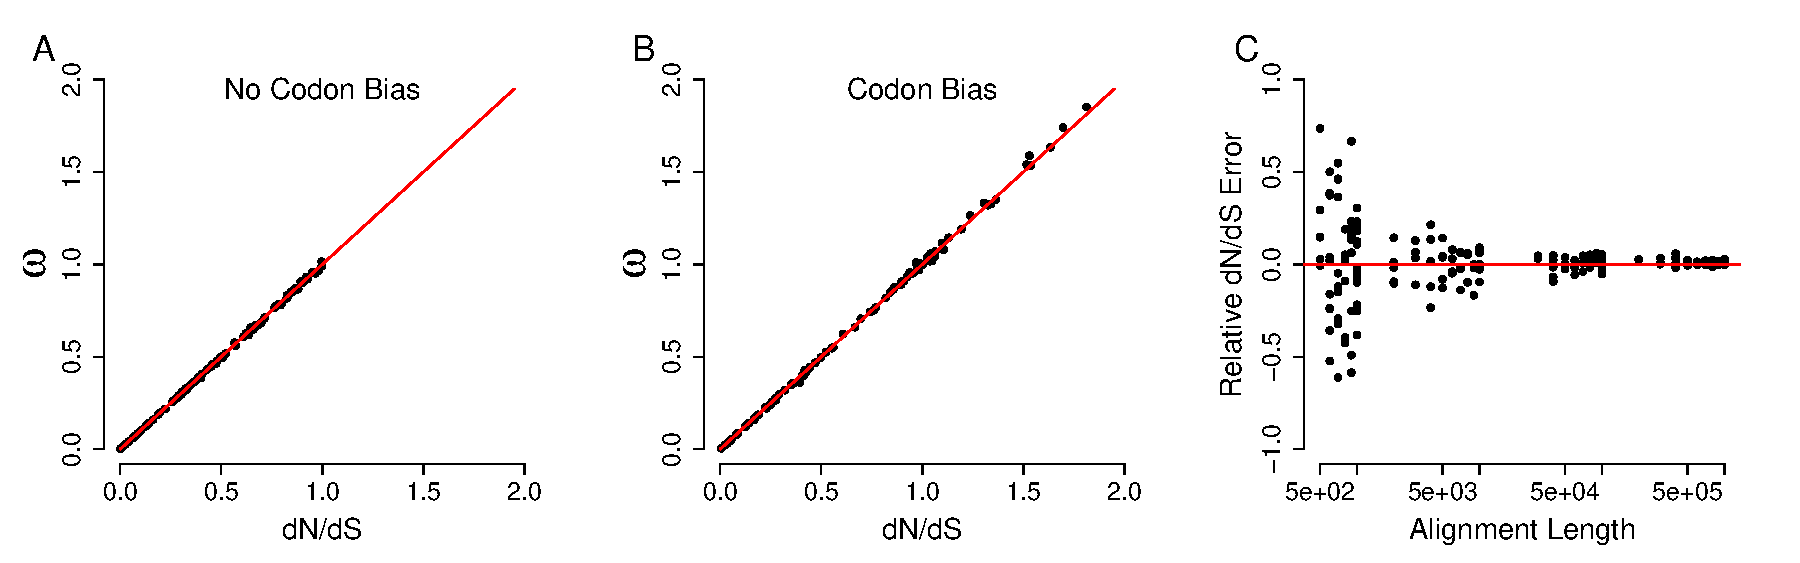
\includegraphics[width=18.7cm]{figures/MainText/regression_convergence.pdf}}
		\caption{\label{reg_conv} Regressions between $dN/dS$ values as calculated from scaled selection coefficients and as inferred using the M0 mechanistic codon model. Each point corresponds to a single simulated alignment. All $\omega$ values shown here were inferred by parameterizing the M0 model with $\kappa$ fixed to its true, simulated value as well as the Fequal codon frequency specification \cite{Yang2006}. The red line in panels (A-B) is the $x=y$ line. (A) Simulations which assigned equal fitness values to synonymous codons ($r^2=0.9995$). (B) Simulations which allowed different fitness values among synonymous codons ($r^2=0.9993$). (C) Convergence of $\omega$ MLEs to the true $dN/dS$ value. The y-axis indicates the relative error of the maximum likelihood $dN/dS$ estimate, and the x-axis indicates the number of positions in the simulated alignment. As the number of positions, and hence the size of the data set, increases, the maximum likelihood estimates converge to the $dN/dS$ values calculated using equations \eqref{eq:pi_i}-\eqref{eq:dS}. The red line in panel (C) is the line $y=0$, indicating no error.}
	\end{figure*}
	
	
	\bigskip
	\bigskip
	\bigskip
	\bigskip
	
	\begin{figure}[htbp]
		\centerline{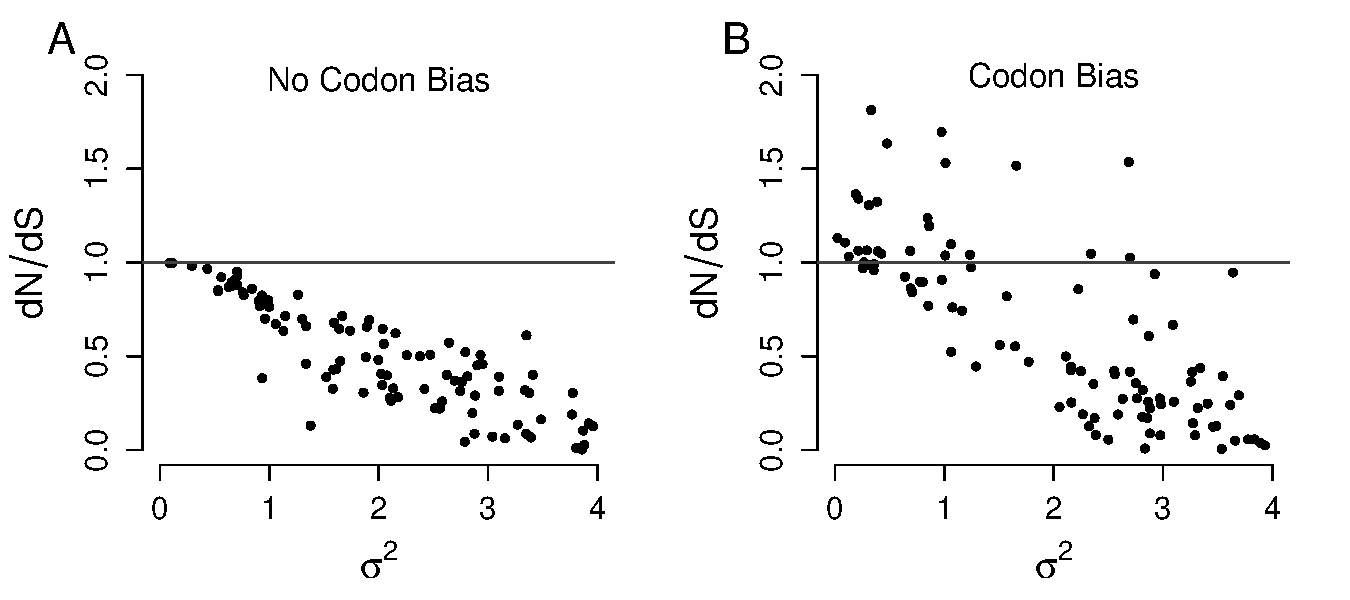
\includegraphics[width=8.7cm]{figures/MainText/sd_vs_dnds.pdf}}
		\caption{\label{stddev_dnds} $dN/dS$ decreases in proportion to amino-acid level selection strength. $dN/dS$ is plotted against the $\sigma^2 $ of the simulated distribution of amino-acid scaled selection coefficients. Higher values of $\sigma^2$ indicate larger fitness differences among amino acids, whereas the limiting value of $\sigma^2 = 0$ means that all amino acids have the same fitness. (A) Simulations which assigned equal fitness values to synonymous codons ($r^2=0.83$). (B) Simulations which allowed different fitness values among synonymous codons ($r^2=0.45$).}
	\end{figure}
	
	\bigskip
	\bigskip
	\bigskip
	\bigskip
	
	\begin{figure}[htbp]
		\centerline{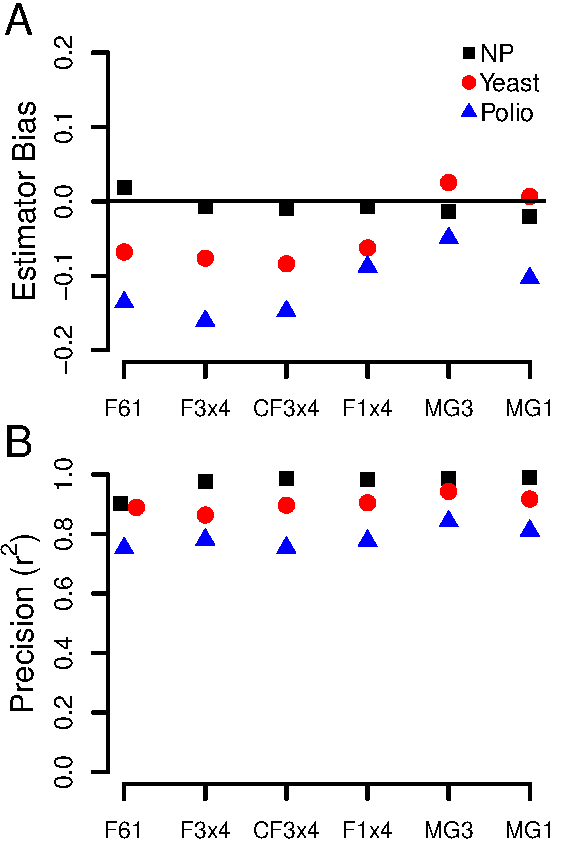
\includegraphics[width=8.7cm]{figures/MainText/nyp_bias_r2.pdf}}
		\caption{\label{nyp_bias_r2} Bias and correlation between $dN/dS$ and $\omega$ MLEs across M0 codon frequency parameterizations, for each set of nucleotide mutation rates. (A) Bias, or systematic deviation from a 1:1 relationship. (B) $r^2$ values between $dN/dS$ and $\omega$. All bias and $r^2$ values are highly statistically significant, with all $p < 10^{-12}$.}
	\end{figure}
	
	\clearpage
	\newpage
	
	\section{Supplementary Information}
	
	\bigskip
	\bigskip
	\bigskip
	\bigskip
	
		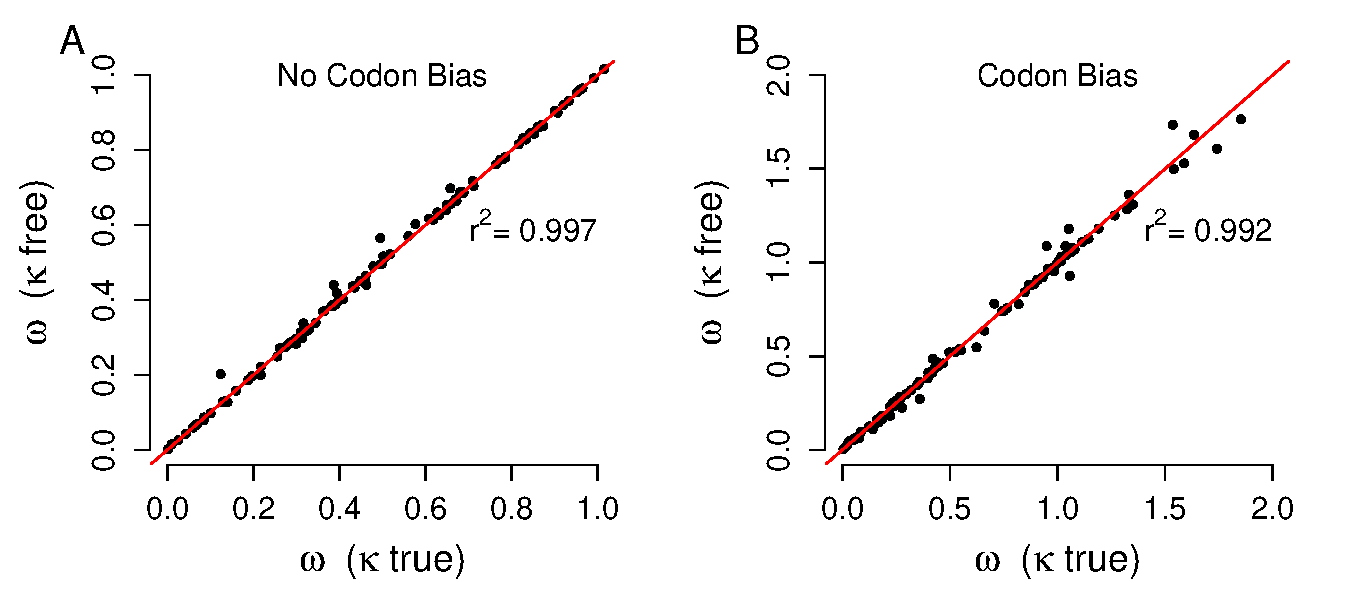
\includegraphics[width=5.5in]{figures/SI/omega_kappafree_kappatrue.pdf}
		\noindent Figure S1. $\omega$ MLEs inferred using the M0 model, where the $\kappa$ parameter in the model's instantaneous rate matrix was either fixed to its true value (x-axis) or allowed to be a free parameter of the model (y-axis). Each point represents a single simulated alignment, and the red lines correspond to $x=y$. All inferences were conducted using the Fequal codon frequency parameterization. There is excellent agreement between $\omega$ estimates for both types $\kappa$ parameterizations.

	
	\bigskip
	\bigskip
	\bigskip
	\bigskip
	
	
	\centerline{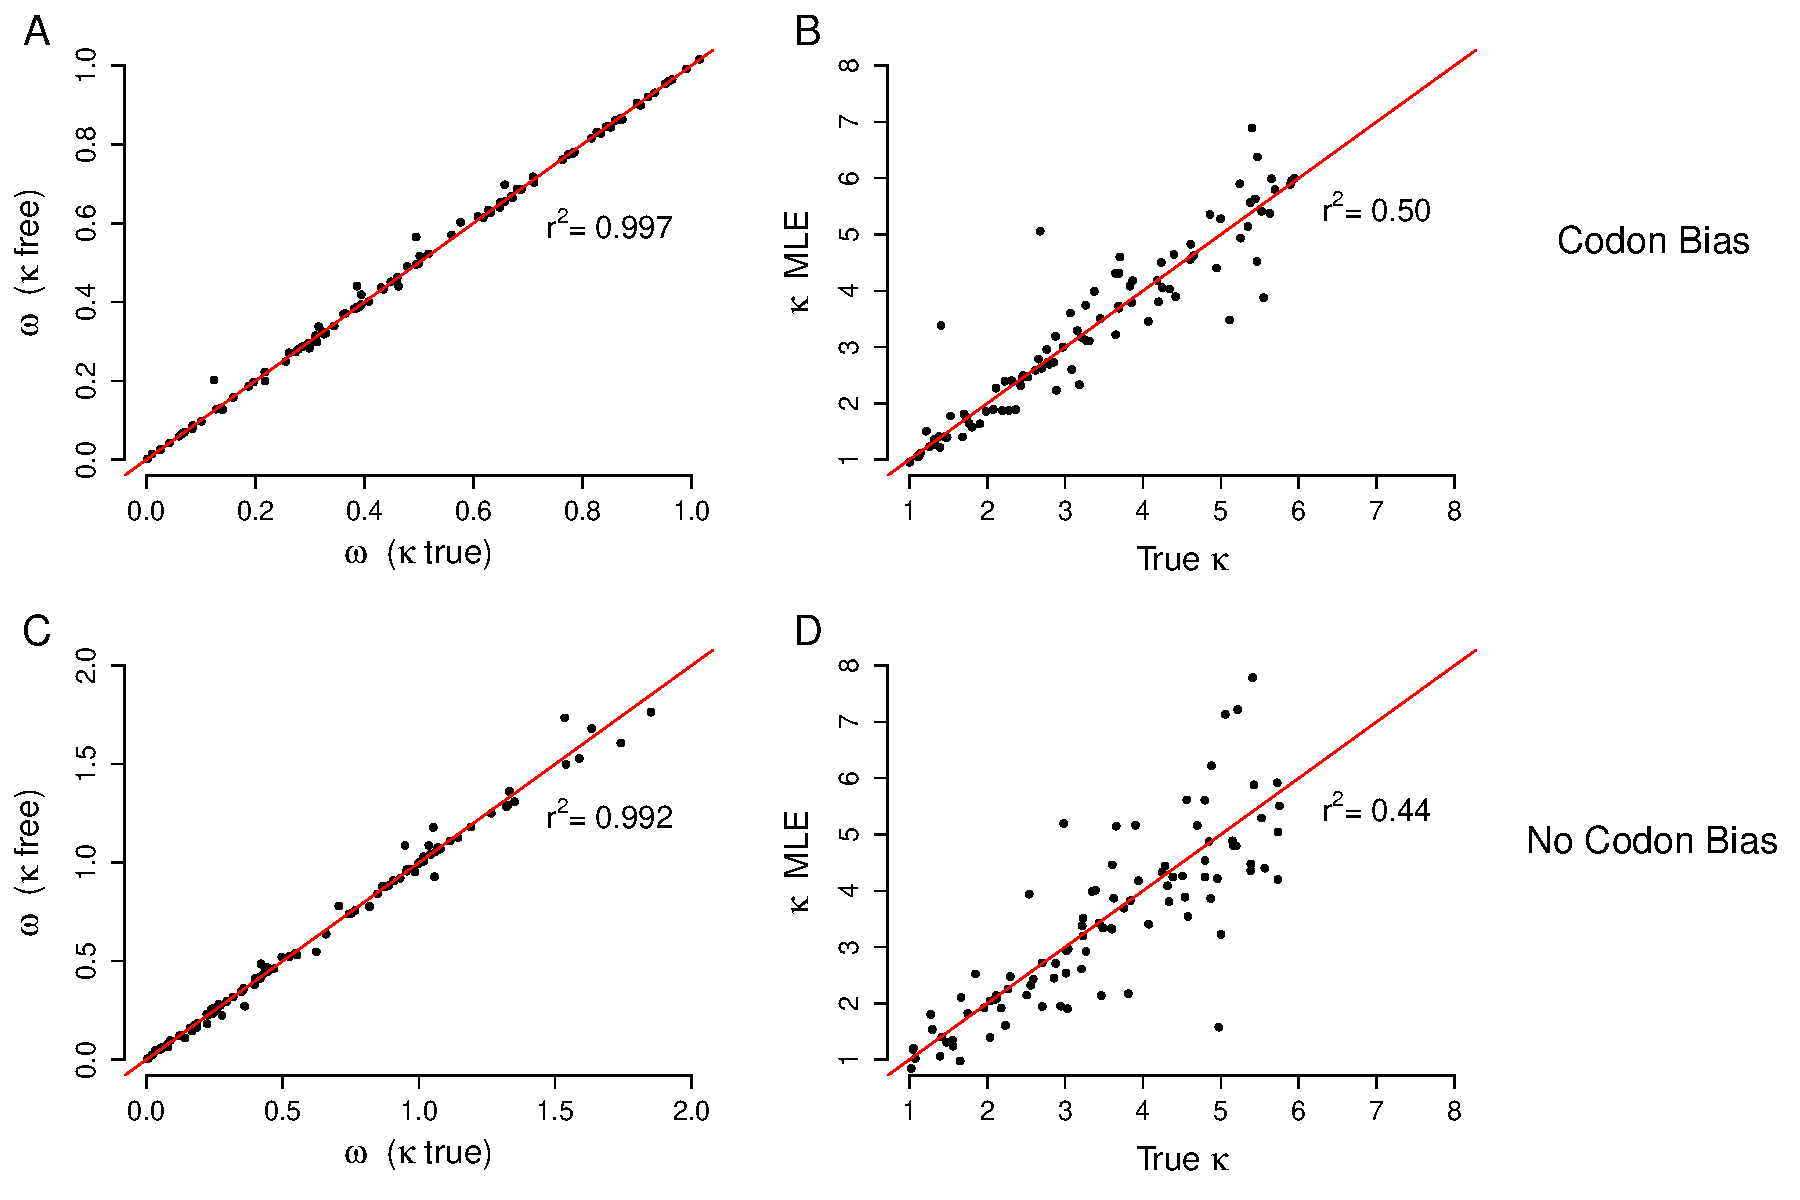
\includegraphics[width=5.5in]{figures/SI/kappa_regressions.pdf}
		\noindent Figure S2. $\kappa$ MLEs are plotted against the true, simulated $\kappa$ values. Each point represents a single simulated alignment, and the red lines correspond to $x=y$. All inferences were conducted using the Fequal codon frequency parameterization. With the exception of a few outlying points, the M0 model yields very accurate $\kappa$ estimates (A) Simulations which assigned equal fitness values to synonymous codons. (B) Simulations which allowed different fitness values among synonymous codons.}
	
	
	\clearpage
	\newpage
	
	\vspace*{-2cm}{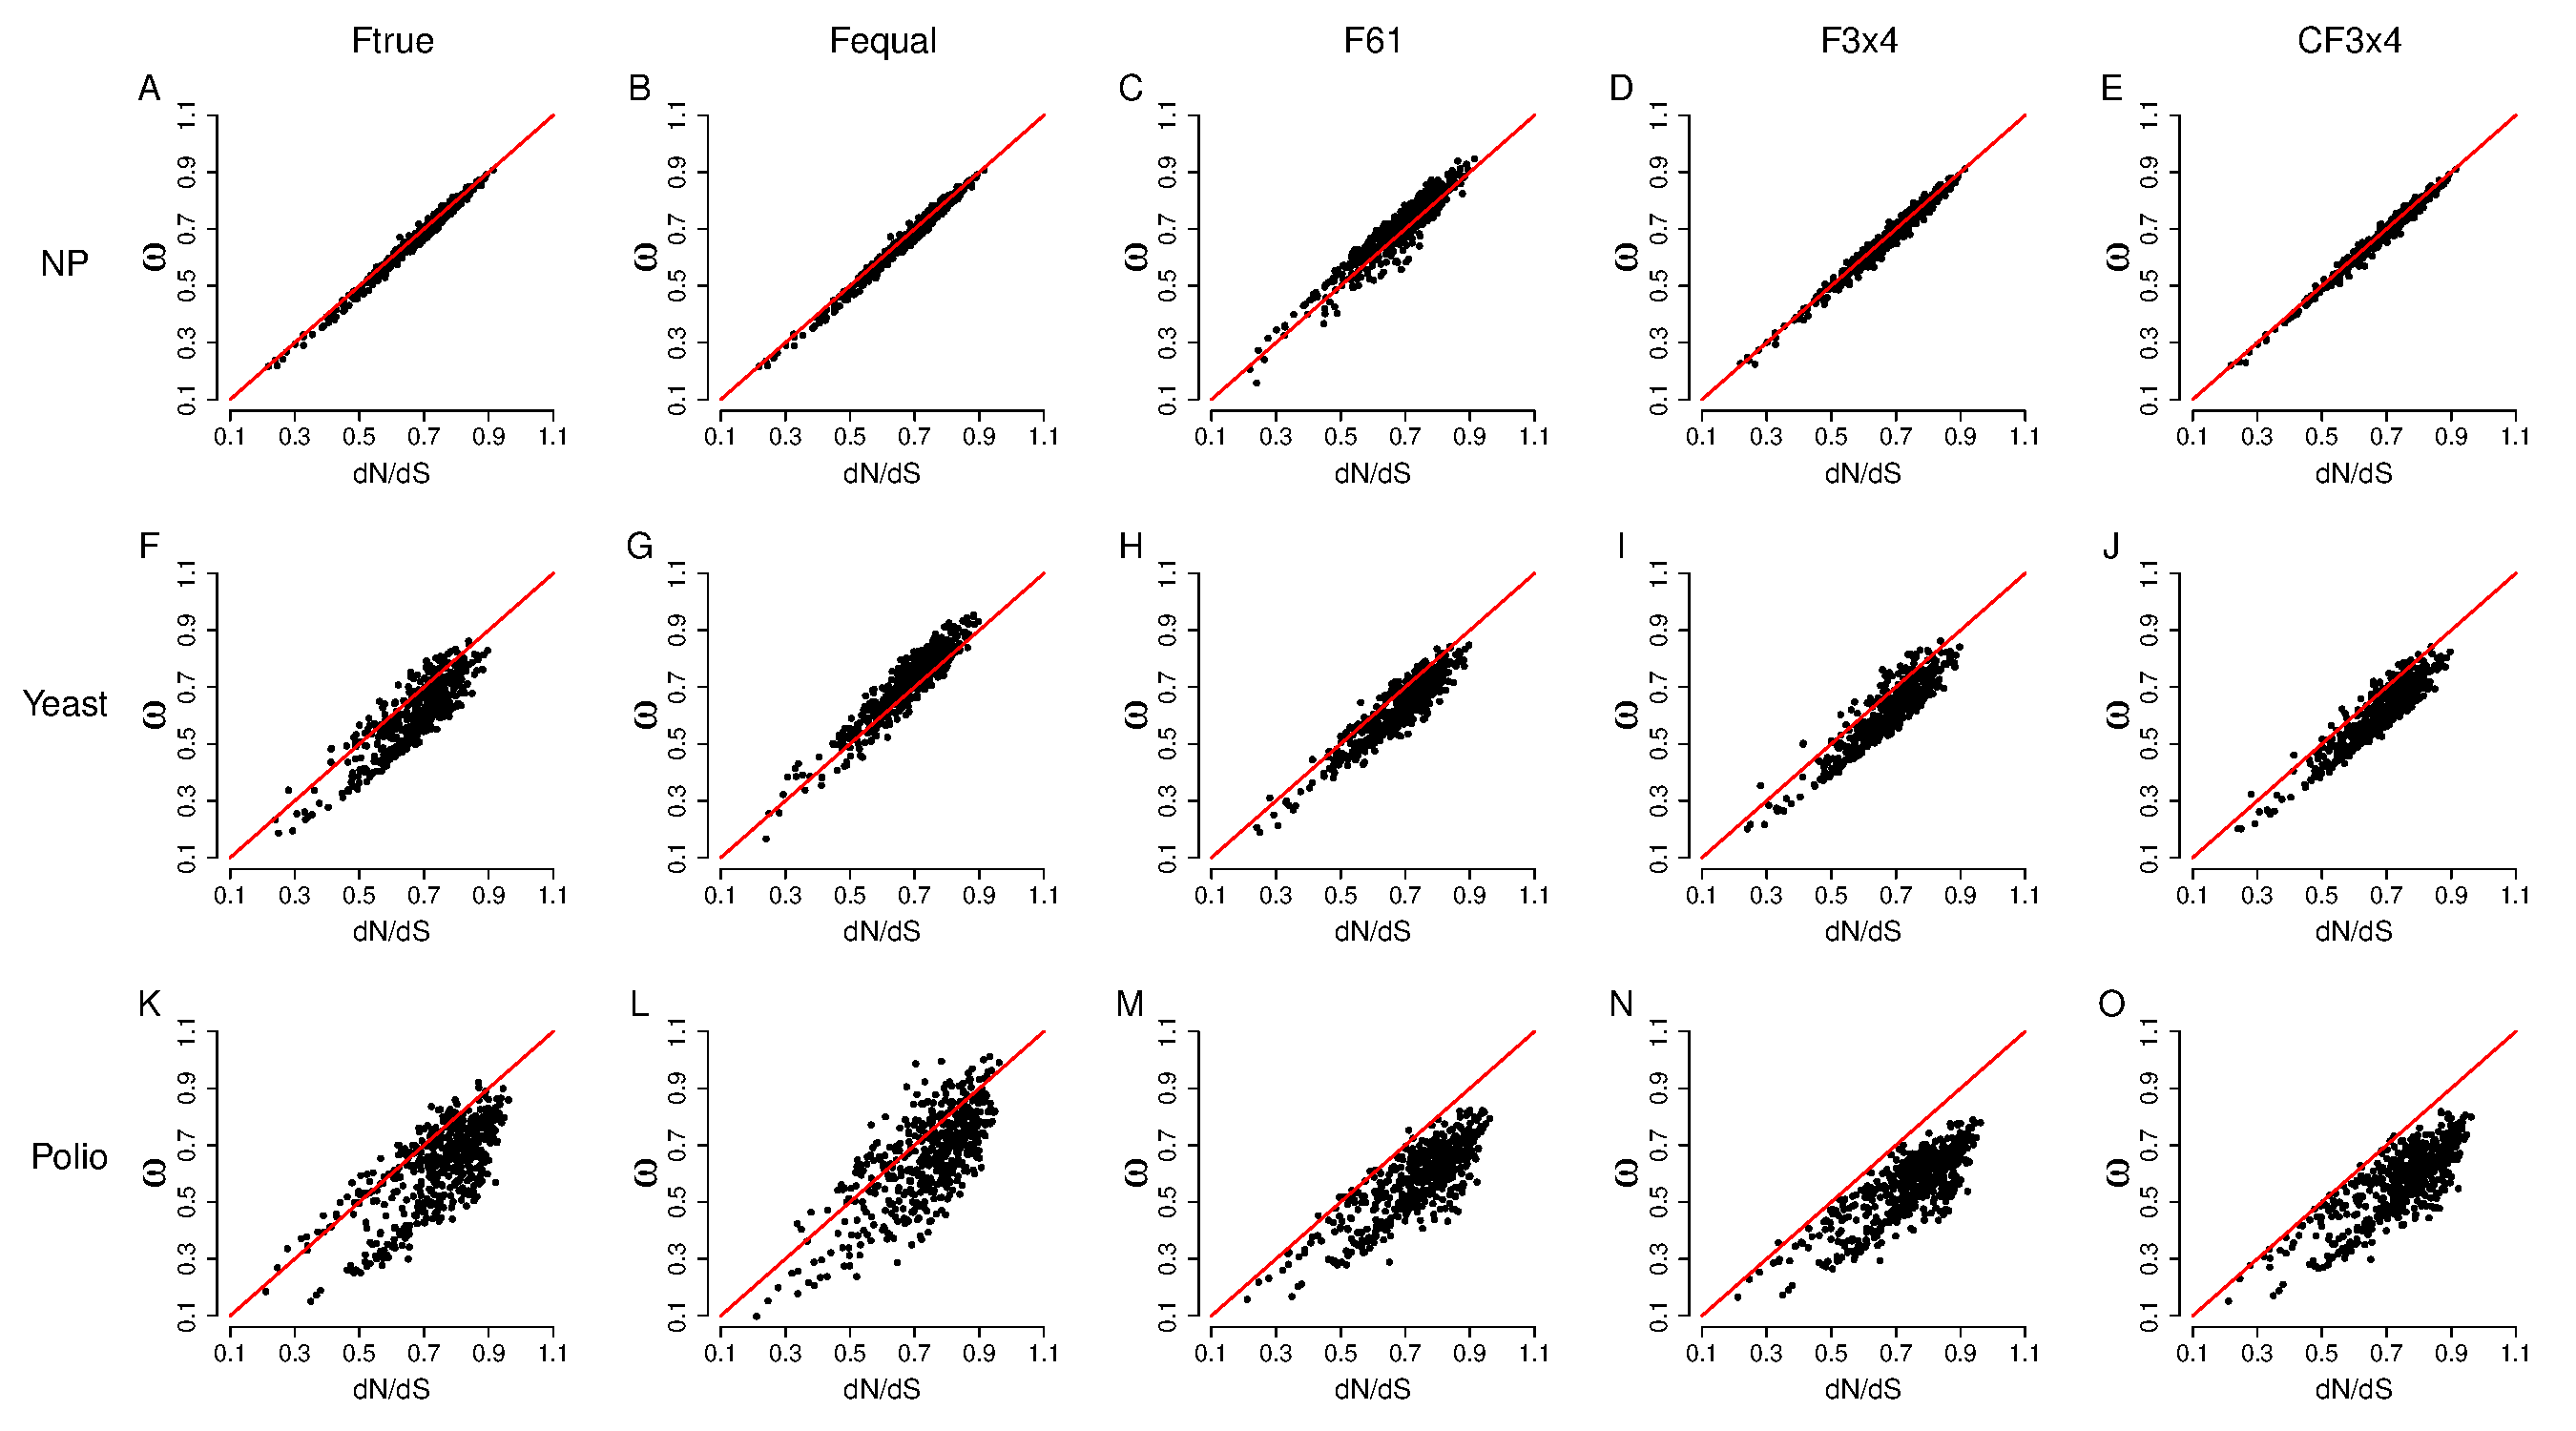
\includegraphics[width=9.25in, angle=90]{figures/SI/nyp_fspecs_full.pdf}
		\noindent Figure S3. Regression plots for $\omega$ MLEs versus $dN/dS$ values computed from scaled selection coefficients, for each set of nucleotide mutation rates and all M0 codon frequency parameterizations. Each point represents a single simulated alignment, and the red lines correspond to $x=y$. (A) Simulations which assigned equal fitness values to synonymous codons. (B) Simulations which allowed different fitness values among synonymous codons.}
	
	\clearpage
	\newpage
	
	
	\noindent Table S1. Estimator bias, representing the mean difference between the expected $dN/dS$ value and estimated $\omega$.  representing the systematic deviation from a 1:1 relationship, between $\omega$ MLEs and $dN/dS$, for all mutation rates and M0 codon frequency parameterizations examined. Negative bias values indicate that $\omega$ MLEs are, on average, lower than $dN/dS$. All biases are statistically significant, with all $p < 10^{-12}$.
	\begin{table}[htbp]
		\begin{tabular}{c c c c c c}
			\hline\noalign{\smallskip}
			& \multicolumn{5}{c}{M0 model codon frequency parameterization} \\
			\cline{2-6}\noalign{\medskip}
			Mutation rate & Ftrue & Fequal & F61 & F3x4 & CF3x4 \\
			\hline\noalign{\smallskip}
			NP & -0.0097 & -0.011 & 0.02 & -0.0063 & -0.0084 \\
			Yeast & -0.072 & 0.029 & -0.056 & -0.066 & -0.073 \\
			Polio & -0.12 & -0.082 & -0.16 & -0.18 & -0.17 \\
			\noalign{\smallskip}\hline\noalign{\smallskip}
		\end{tabular}
	\end{table}	
	
	\bigskip
	\bigskip
	\bigskip
	\bigskip
	\bigskip
	
	\noindent Table S2. NYP $r^2$ values between $\omega$ MLEs and $dN/dS$, for all mutation rates and M0 codon frequency parameterizations examined. All $r^2$ values are statistically significant, with all $p < 10^{-15}$.
	\begin{table}[htbp]
		\begin{tabular}{c c c c c c}
			\hline\noalign{\smallskip}
			& \multicolumn{5}{c}{M0 model codon frequency parameterization} \\
			\cline{2-6}\noalign{\medskip}
			Mutation rate & Ftrue & Fequal & F61 & F3x4 & CF3x4 \\
			\hline\noalign{\smallskip}
			NP & 0.988 & 0.986 & 0.902 & 0.975 & 0.986 \\
			Yeast & 0.740 & 0.877 & 0.850 & 0.820 & 0.848 \\
			Polio & 0.537 & 0.519 & 0.659 & 0.671 & 0.641 \\
			\noalign{\smallskip}\hline\noalign{\smallskip}
		\end{tabular}
	\end{table}	
	
\end{document}

